\section{Product perspesctive}
\label{sec:product_perspesctive}%

\subsection{Scenarios}
\label{subsec:scenarios}%

% ======================
% 1. AUTHENTICATION AND ACCESS
% ======================
\subsubsection{Authentication and Access Scenarios}
\newcounter{aac}
\setcounter{aac}{1}
\newcommand{\caac}{\theaac\stepcounter{aac}}

\begin{center}
    \begin{longtable}{@{}|p{0.19\linewidth}|p{0.81\linewidth}|@{}}
        \hline
        \textbf{Scenario ID} & \textbf{1.\caac – Registration (Success)} \\
        \hline
        \textbf{Actor} & Anna (new user) \\
        \hline
        \textbf{Preconditions} & Internet connection available (\hyperref[da:12]{DA12}). \\
        \hline
        \textbf{Description} & Anna opens the BBP app and taps “Register.” She enters her email and password. Upon confirmation, the system creates the account, authenticates her, and redirects her to the main map screen as a registered user. \\
        \hline
        \textbf{Postconditions} & The user account is created, and Anna is logged in. \\
        \hline
        \end{longtable}
\end{center}

\begin{center}
    \begin{longtable}{@{}|p{0.19\linewidth}|p{0.81\linewidth}|@{}}
        \hline
        \textbf{Scenario ID} & \textbf{1.\caac – Login (Success)} \\
        \hline
        \textbf{Actor} & Carlo (registered user) \\
        \hline
        \textbf{Preconditions} & Valid credentials and Internet connection (\hyperref[da:12]{DA12}). \\
        \hline
        \textbf{Description} & Carlo opens the app, selects “Login,” enters his credentials (“CarloMTB,” password), and presses “Sign In.” The BBP system verifies them and grants access, showing the main map screen. \\
        \hline
        \textbf{Postconditions} & Carlo is authenticated and redirected to the main map screen. \\
        \hline
    \end{longtable}
\end{center}

\newpage

\begin{center}
    \begin{longtable}{@{}|p{0.19\linewidth}|p{0.81\linewidth}|@{}}
        \hline
        \textbf{Scenario ID} & \textbf{1.\caac – Login (Exception – Wrong Password)} \\
        \hline
        \textbf{Actor} & Carlo (registered user) \\
        \hline
        \textbf{Preconditions} & Incorrect password entered. \\
        \hline
        \textbf{Description} & Carlo tries to log in but mistypes his password. The BBP system verifies the credentials and, upon failure, shows an error message: “Invalid username or password,” keeping him on the login page. \\
        \hline
        \textbf{Postconditions} & Login fails; no session is created. \\
        \hline
    \end{longtable}
\end{center}

% ======================
% 2. ROUTE CONSULTATION
% ======================

\subsubsection{Route Consultation Scenarios}
\newcounter{rcs}
\setcounter{rcs}{1}
\newcommand{\crcs}{\thercs\stepcounter{rcs}}

\begin{center}  
    \begin{longtable}{@{}|p{0.19\linewidth}|p{0.81\linewidth}|@{}}
        \hline
        \textbf{Scenario ID} & \textbf{2.\crcs – Search and Display (Success)} \\
        \hline
        \textbf{Actor} & Marco (anonymous user) \\
        \hline
        \textbf{Preconditions} & Internet connection available (\hyperref[da:12]{DA12}). \\
        \hline
        \textbf{Description} & Marco uses the search bar to set “Stazione Garibaldi” as the origin and “Parco di Monza” as the destination. The BBP system processes the query, computes route scores, and shows an ordered list. Marco selects “Route A,” and the app displays the route, details (distance, elevation), and weather forecast (\hyperref[da:11]{DA11}). \\
        \hline
        \textbf{Postconditions} & Routes are displayed; user views the selected route and related data. \\
        \hline
    \end{longtable}
\end{center}

\begin{center} 
    \begin{longtable}{@{}|p{0.19\linewidth}|p{0.81\linewidth}|@{}}
        \hline
        \textbf{Scenario ID} & \textbf{2.\crcs – System Logic (Scoring \& Merging) – Key Scenario} \\
        \hline
        \textbf{Actor} & BBP System \\
        \hline
        \textbf{Preconditions} & User search triggered (Scenario 2.1). Data from past route reports available (\hyperref[da:8]{DA8})(\hyperref[da:9]{DA9}). \\
        \hline
        \textbf{Description} & “Route B” has three status updates: two “Requires Maintenance” and one “Optimal.” The system’s merging algorithm aggregates the data based on freshness (\hyperref[da:8]{DA8} and majority (\hyperref[da:9]{DA9}), assigning “Requires Maintenance.” The scoring algorithm uses this to compute a final score of 6.5. \\
        \hline
        \textbf{Postconditions} & Aggregated route status and updated score are displayed to the user. \\
        \hline
    \end{longtable}
\end{center}

\begin{center} 
    \begin{longtable}{@{}|p{0.19\linewidth}|p{0.81\linewidth}|@{}}
        \hline
        \textbf{Scenario ID} & \textbf{2.\crcs – Search (Exception – No Route Found)} \\
        \hline
        \textbf{Actor} & Marco (anonymous user) \\
        \hline
        \textbf{Preconditions} & Query between remote or unsupported locations. \\
        \hline
        \textbf{Description} & Marco searches for a route, but no publishable results match the criteria. The BBP system displays: “No BBP route found. Be the first to create one!” \\
        \hline
        \textbf{Postconditions} & No results displayed; user invited to create a route. \\
        \hline
    \end{longtable}
\end{center}

\begin{center} 
    \begin{longtable}{@{}|p{0.19\linewidth}|p{0.81\linewidth}|@{}}
        \hline
        \textbf{Scenario ID} & \textbf{2.\crcs – Navigation} \\
        \hline
        \textbf{Actor} & Marco (anonymous user) \\
        \hline
        \textbf{Preconditions} & A route has been selected. Accurate GPS assumed (\hyperref[da:2]{DA2}). \\
        \hline
        \textbf{Description} & Marco presses “Follow Route.” The app loads the route and shows his real-time position using GPS. The system guides him along the route without recording a new one. At the end, the system offers to register Marco so he can save his ride or view only trip data. \\
        \hline
        \textbf{Postconditions} & Trip completed; user may register or view data summary. \\
        \hline
    \end{longtable}
\end{center}


% ======================
% 3. ROUTE CREATION
% ======================

\subsubsection{Route Creation Scenarios}
\newcounter{rc}
\setcounter{rc}{1}
\newcommand{\crc}{\therc\stepcounter{rc}}

\begin{center} 
    \begin{longtable}{@{}|p{0.19\linewidth}|p{0.81\linewidth}|@{}}
       \hline
        \textbf{Scenario ID} & \textbf{3.\crc – Manual Route Creation (Success)} \\
        \hline
        \textbf{Actor} & Anna (registered user) \\
        \hline
        \textbf{Preconditions} & User logged in; understands options (\hyperref[da:10]{DA10}). \\
        \hline
        \textbf{Description} & From her profile, Anna selects “Create Manual Route.” She draws the route on the map, names it “Tuesday Ride,” places maintenance pins, activates “Make Public,” and presses “Save” (\hyperref[da:2]{DA2}). The route becomes available to others. \\
      \hline
     \textbf{Postconditions} & The new route is created and visible to all users. \\
       \hline
    \end{longtable}
\end{center}

\newpage

\begin{center}
    \begin{longtable}{@{}|p{0.19\linewidth}|p{0.81\linewidth}|@{}}
        \hline
        \textbf{Scenario ID} & \textbf{3.\crc – Automatic Recording (Success \& Pothole Detection) – Key Scenario} \\
        \hline
        \textbf{Actor} & Carlo (registered user) \\
        \hline
        \textbf{Preconditions} & Accurate GPS data (\hyperref[da:2]{DA2}), reliable threshold (\hyperref[da:4]{DA4}), device fixed to bike (\hyperref[da:5]{DA5}). \\
        \hline
        \textbf{Description} & Carlo presses “Start Recording.” The app tracks his movement, displaying real-time data. While riding, a strong shock occurs due to a pothole. Sensors send data spikes to BBP. Upon completion, BBP asks for confirmation; Carlo validates correct detections and saves the trip. The app displays weather data (\hyperref[da:11]{DA11}) and summary before saving (\hyperref[da:12]{DA12}). \\
        \hline
        \textbf{Postconditions} & Trip data and confirmed detections are stored in Carlo’s archive. \\
        \hline
    \end{longtable}
\end{center}

\begin{center}
    \begin{longtable}{@{}|p{0.19\linewidth}|p{0.81\linewidth}|@{}}
       \hline
        \textbf{Scenario ID} & \textbf{3.\crc – Automatic Recording (False Detection \& User Correction)} \\
        \hline
        \textbf{Actor} & Carlo (registered user) \\
        \hline
        \textbf{Preconditions} & Same as Scenario 3.2; false detection occurs. \\
        \hline
        \textbf{Description} & Carlo’s recording continues, but the detected spike results from jumping off a curb. When asked to confirm detections, Carlo (acting in good faith, (\hyperref[da:7]{DA7})) presses “No, ignore” for incorrect ones. The BBP system cancels invalid detections, and Carlo completes the trip as in Scenario 3.2. \\
        \hline
        \textbf{Postconditions} & False detections are removed; valid trip data saved. \\
        \hline
    \end{longtable}
\end{center}

\begin{center}
    \begin{longtable}{@{}|p{0.19\linewidth}|p{0.81\linewidth}|@{}}
        \hline
        \textbf{Scenario ID} & \textbf{3.4 – Automatic Recording (No Detections)} \\
        \hline
        \textbf{Actor} & Carlo (registered user) \\
        \hline
        \textbf{Preconditions} & Flat and obstacle-free route; no sensor spikes (\hyperref[da:4]{DA4}). \\
        \hline
        \textbf{Description} & Carlo rides on a smooth route. No anomalies are detected. When pressing “End and Save,” BBP skips the “Review” step and directly shows the summary screen. \\
        \hline
        \textbf{Postconditions} & Trip saved successfully without detected issues. \\
        \hline
    \end{longtable}
\end{center}

\newpage

\subsection{Class diagrams}
\label{subsec:class_diagrams}%


\begin{figure}[H]
    \begin{center}
        
\includegraphics[width=0.9\linewidth]{UML_Class_Diagram.png}
        \caption{High level Class Diagram.}
        \label{fig:UML}%
    \end{center}
\end{figure}



\section*{Class Diagram Description}
\label{subsec:class_diagram_description} % Optional label for cross-referencing

The system's structure revolves around the base \textbf{User} entity. The \texttt{Registered\_user} class extends \texttt{User}, incorporating attributes like \texttt{username}, \texttt{email}, and \texttt{passwordHash} necessary for authentication and user identification. Each registered user is associated with their recorded activities and contributions.

A core distinction is made between a \texttt{Trip} and a \texttt{Path}. A \texttt{Trip} represents a specific, private cycling session recorded by a \texttt{Registered\_user}. It is fundamentally defined as a composition of multiple \texttt{GPS\_points}, each containing latitude, longitude, and a timestamp, thus capturing the entire journey. Furthermore, each \texttt{Trip} is linked via composition to exactly one \texttt{Statistic} object (holding calculated data like \texttt{avg\_speed}, \texttt{distance}, \texttt{duration}) and associated with one \texttt{Weather\_info} object (containing \texttt{temperature}, \texttt{wind\_speed}, \texttt{conditions}) obtained from external sources.

Conversely, the \texttt{Path} class represents a public, discoverable route, potentially derived from a user's \texttt{Trip} or created manually. Like a \texttt{Trip}, it is composed of \texttt{GPS\_points} defining its geometry. Crucially, a \texttt{Path} serves as an aggregation point for community feedback, being associated with multiple \texttt{Report} instances. The \texttt{<<Abstract>> Report} class acts as the base for all user-submitted information regarding a \texttt{Path}, containing a vital \texttt{timestamp} attribute used for the merging algorithm's "freshness" logic. It has two concrete specializations:
\begin{itemize}[noitemsep, topsep=0pt]
    \item \texttt{Status\_report}: Captures user assessments of the path's condition via the \texttt{<<Enum>> status} attribute (e.g., ``Optimal'', ``Requires Maintenance'').
    \item \texttt{Obstacle\_report}: Represents specific issues like potholes, categorized by an \texttt{<<Enum>> type}. Importantly, it maintains a \texttt{[0..1]} association with a \texttt{sensor\_event}, linking a confirmed report back to the raw sensor data that potentially triggered its detection.
\end{itemize}

The \texttt{sensor\_event} class models the raw detection triggered by device sensors (accelerometer/gyroscope) during a \texttt{Trip}, storing its location and timestamp before user confirmation. The interaction with external systems (conceptually noted, though not modeled as domain classes) like device sensors and weather services is fundamental for data acquisition.

Overall, the diagram establishes a clear architecture separating \textbf{user management}, private \textbf{trip recording} with detailed metrics, public \textbf{path representation}, and a structured \textbf{reporting system} capable of handling community feedback and sensor-based obstacle detection through inheritance.



\subsection{State diagrams}
\label{subsec:state_diagrams}%
In this section, the State Diagrams of the BBP system are presented representing all the possible operation that a User can perform.
\paragraph{Signup.}
When a user opts to register for BBP, they are initially presented with the registration option on the interface. Upon tapping the registration button, the system displays the dedicated registration screen. The user then enters the required credentials, such as username, email, and password. Subsequently, BBP performs a check to validate the provided information. If the credentials are deemed valid, the registration is successful, and the user is navigated to the main map screen. However, if the validation fails (due to invalid format or existing username/email), the flow loops back, presumably returning the user to the registration screen to correct their input and try again.


\begin{figure}[H]
    \begin{center}
        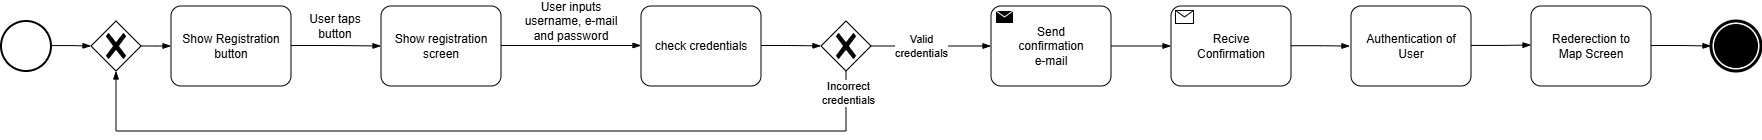
\includegraphics[width=1\linewidth]{RASD/LaTeXCode/images/StateDiagrams/Registration.drawio.png}
        \caption{Registration state diagram.}
        \label{fig:signup_sd}%
    \end{center}
\end{figure}

\newpage

\paragraph{Login.}
When a registered User attempts to log in to their BBP account, they must enter their credentials (nickname and password) into a login form. If the provided credentials are accurate —matching those of a registered User in the BBP database— BBP authenticates the User and redirects him to the Map Screen, showcasing the possibility to discover new path. however, if the entered credentials are invalid, BBP presents an error message to the User and redirects them back to the login form page.

\begin{figure}[H]
    \begin{center}
        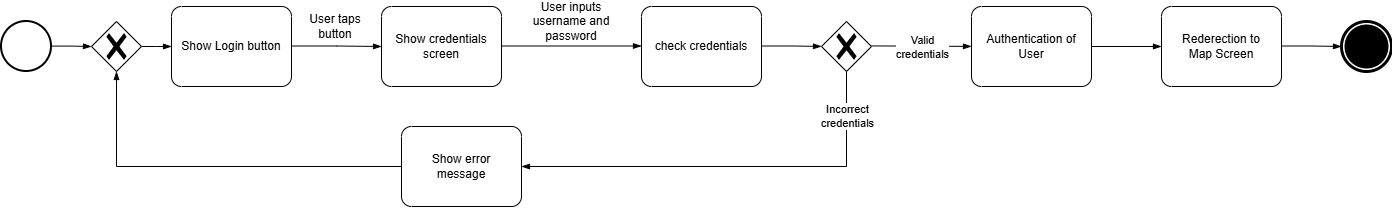
\includegraphics[width=1\linewidth]{RASD/LaTeXCode/images/StateDiagrams/Login.drawio.png}
        \caption{Login state diagram.}
        \label{fig:login_sd}%
    \end{center}
\end{figure}

\paragraph{Search and Display.}
When an anonymous user intends to look up a route on BBP, he is required to provide an origin and a destination in the search form. If an Internet connection is available, BBP processes the submitted query, computes route scores, and prepares an ordered list of publishable results. If at least one result is available, BBP displays the ordered list; after the User selects a route (e.g., “Route A”), the system shows the route on the map together with its details (distance, elevation) and the weather forecast.

In contrast, if no publishable route matches the criteria—for example, when the query concerns remote or unsupported locations—BBP informs Marco with the message “No BBP route found. Be the first to create one!” and no results are shown.

\begin{figure}[H]
    \begin{center}
        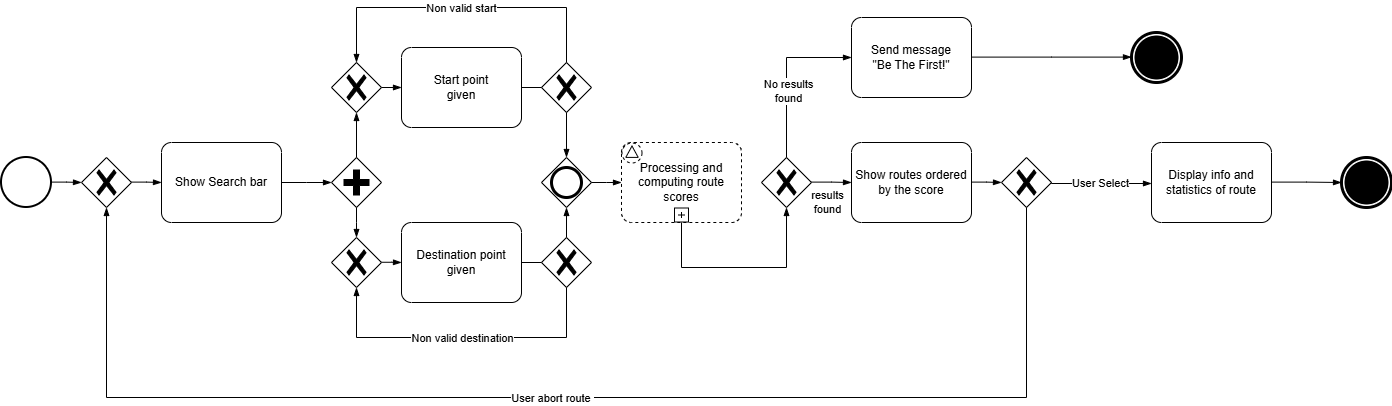
\includegraphics[width=1\linewidth]{RASD/LaTeXCode/images/StateDiagrams/SearchAndDisplay.drawio.png}
        \caption{Search and Display state diagram.}
        \label{fig:Search_And_Display_sd}%
    \end{center}
\end{figure}

\newpage

\paragraph{Scoring \& Merging.}
When a route search is triggered (Scenario 2.1), the BBP System gathers the past route reports for the selected route (DA8/DA9) and verifies that the data are available and readable. The system then applies the merging logic: a majority rule over the collected statuses (DA9). If a majority tie occurs, the system resolves it using the freshness criterion, giving precedence to the most recent and reliable reports (DA8). If the data are missing, corrupted, or a tie remains unresolvable, BBP notifies the user (e.g., “No data available” or “Conflict in reports”) and aborts the update.

Conversely, when a merged status is successfully determined, the scoring algorithm computes the route’s numeric score (e.g., 6.5) based on the merged outcome and recency weighting. The aggregated status and computed score are then presented to the user and logged for traceability. Any failure during fetching, merging, scoring, or presentation results in an error message and termination of the operation without altering previously displayed results.

\begin{figure}[H]
    \begin{center}
        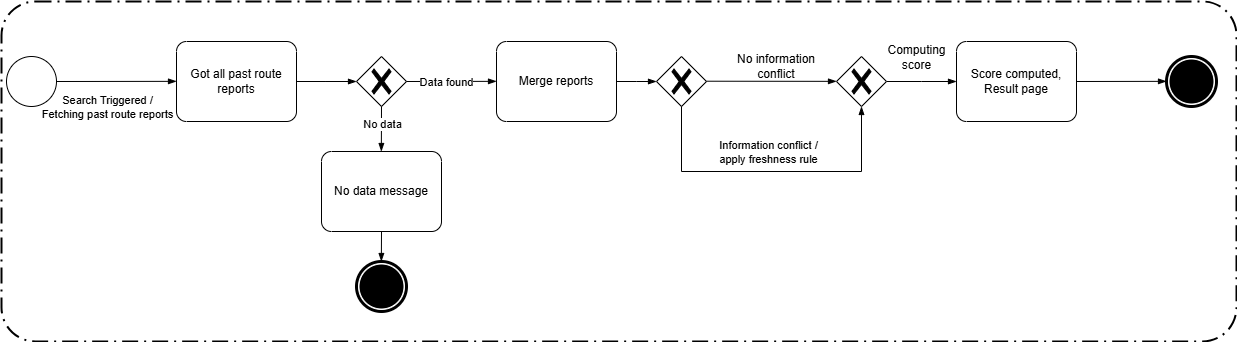
\includegraphics[width=1\linewidth]{RASD/LaTeXCode/images/StateDiagrams/Scoring&MergingLogic.drawio.png}
        \caption{Scoring \& Merging logic state diagram.}
        \label{fig:Scoring_Merging_sd}%
    \end{center}
\end{figure}

\paragraph{Navigation.}
After a route has been selected, the User taps \emph{Follow Route}. The BBP system loads the chosen route and begins step-by-step guidance using his current position (GPS assumed to be always available). While guiding, the system continuously checks adherence to the planned path;
%TODO bagai qua in caso non lo assumiamo come vero rimettimao
%if a deviation is detected, it recenters the view and proposes a reroute, then resumes guidance on the corrected path.
When the User reaches the destination, BBP displays an end-of-trip screen offering registration. If the Anonymous User chooses to register, BBP saves the trip to their account and then displays the trip summary; otherwise, BBP simply presents a view-only summary without storing the ride.

Conversely, if the User is already registered, the trip is automatically saved, and the Authenticated User can choose to view the summary or exit the navigation.

\begin{figure}[H]
    \begin{center}
        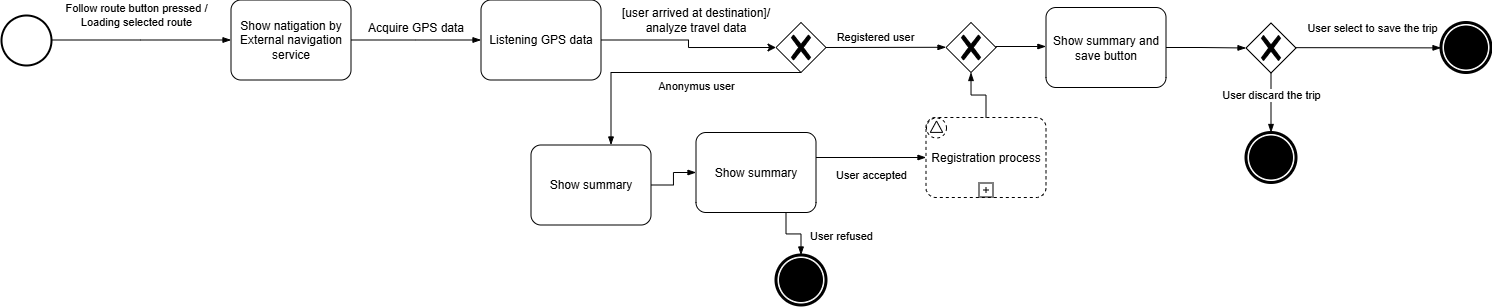
\includegraphics[width=1\linewidth]{RASD/LaTeXCode/images/StateDiagrams/Navigation.drawio.png}
        \caption{Navigation state diagram.}
        \label{fig:Navigation_sd}%
    \end{center}
\end{figure}

\paragraph{Manual Route Creation.}
From the User's profile, User opens the \emph{Manual Route Editor}. Once the editor is ready, he iteratively builds the path by adding/undoing segments until the path is marked complete. At completion, the system processes the geometry (e.g., distance and altitude) and then prompts for optional maintenance pins; The User may add any number of pins before proceeding. Next, he attaches metadata—entering the route name and selecting the visibility (Public/Private)—and presses \emph{Save}. The system validates the submission (path present and consistent metadata). If validation fails, the flow terminates without saving and feedback is shown. If validation succeeds, the system checks the visibility setting: when \emph{Public} is allowed and selected, the route is published and indexed for all users; otherwise, the route is saved privately in the User’s library. The process then ends.

\begin{figure}[H]
    \begin{center}
        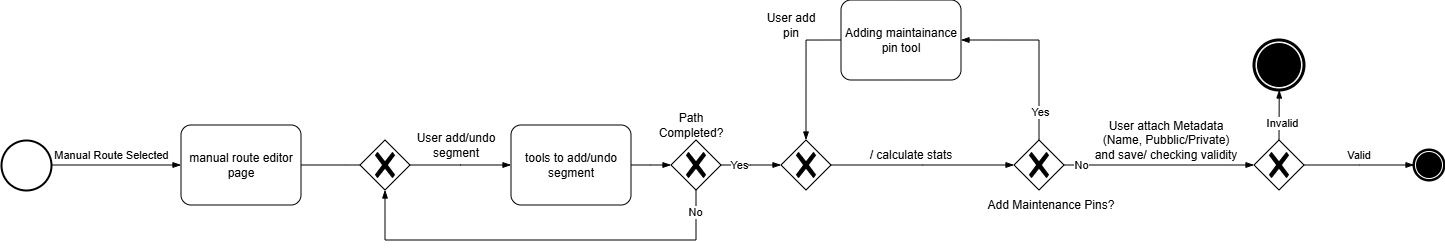
\includegraphics[width=1\linewidth]{RASD/LaTeXCode/images/StateDiagrams/ManualRouteCreation.drawio.png}
        \caption{Manual Route Creation state diagram.}
        \label{fig:Manual_Route_Creation_sd}%
    \end{center}
\end{figure}

\paragraph{Automatic Route Creation.}
When the User presses \emph{Start Recording}, BBP initializes the session, updates the HUD, and activates sensors. In parallel, GPS data are retrieved to build the path. While the session is active, each shock above the detection threshold is logged as a \emph{pending detection} and the ride continues. When the User presses \emph{End}, the system elaborates the path (e.g., distance and elevation) and checks whether a review is required (\texttt{pendingDetections > 0}). If a review is needed, the User confirms or rejects every candidate; only confirmed detections are retained. BBP then computes the trip summary \& weather information, stores the trip (with confirmed detections), and finally displays the summary screen.

\begin{figure}[H]
    \begin{center}
        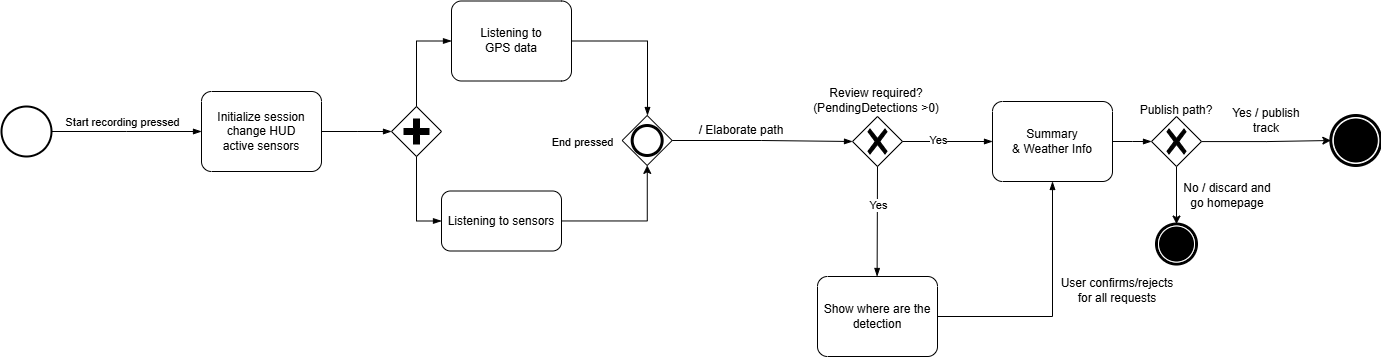
\includegraphics[width=1\linewidth]{RASD/LaTeXCode/images/StateDiagrams/AutomaticRecording.drawio.png}
        \caption{Automatic Recording state diagram.}
        \label{fig:Automatic_Recording_sd}%
    \end{center}
\end{figure}


\section{Product functions}
\label{sec:product_functions}%

Here are listed a summary of the main functions of the BBP system:\\\\

\textbf{Signup:} The User enters email and password to create a new BBP account; a confirmation email completes activation and the User is redirected to the map as a registered user.\\
\textbf{Login:} The User types credentials (nickname/email and password); if valid, BBP starts the session and shows the main map; otherwise, an error is shown and the User remains on the login page.\\
\textbf{Logout:} The User ends the current session; subsequent access requires logging in again.\\
\textbf{Search Route:} The User specifies origin and destination; BBP computes scores and returns an ordered list of publishable routes.\\
\textbf{View Route Details:} After selecting a route, BBP displays the polyline, distance, elevation, and the weather forecast associated with the route.\\
\textbf{Follow Route (Navigation):} The User taps “Follow Route”; BBP provides turn-by-turn guidance using GPS without recording a new trip. At the end, BBP offers registration so the User can save the ride or view a summary only.\\
\textbf{Start Automatic Recording:} A registered User starts a session; BBP tracks the path and live stats while acquiring motion-sensor data (accelerometer/gyroscope).\\
\textbf{Automatic Detection Review:} At the end of recording, BBP asks the User to confirm or reject sensor-detected anomalies (e.g., potholes); only confirmed detections are retained.\\
\textbf{End \& Save Trip:} BBP computes trip statistics and attaches a weather snapshot; the trip (and any confirmed detections) is saved to the User’s archive.\\
\textbf{Manual Route Creation:} The User opens the editor, draws the path, optionally adds maintenance pins, sets name and visibility, and presses “Save.”\\
\textbf{Publish/Privacy Choice:} When saving a manually created route, the User can make it Public (visible to everyone) or keep it Private in their library.\\
\textbf{Route Scoring \& Merging:} For searched paths, BBP aggregates community reports by majority and freshness to derive the current status and compute the route score shown in results.\\
\textbf{My Trips \& Summaries:} Registered Users can view stored trips with summaries (distance, duration, elevation, average speed) and associated weather info.\\
\textbf{Notifications \& Messages:} BBP displays confirmations, success, or error messages during key actions (e.g., save completed, invalid credentials, no route found).\\

\section{User characteristic}
\label{sec:User_characteristic}%

There are two categories of BBP users: Anonymous Users and Registered Users. Their main characteristics:
\begin{itemize}
    \item \textbf{Anonymous User (Guest).} Can use BBP without an account to search for routes between an origin and a destination and visualize them on the map, ranked by score. May follow an existing route (navigation / view-only trip summary), but cannot save rides or publish information. A network connection and location access are required during use.  
    \item \textbf{Registered User.} Creates an account to record and store personal trips, view trip statistics (e.g., total distance, average speed), and—when available—have trips enriched with weather data retrieved from an external service. Can contribute publishable information about bike paths in two ways: (i) manual mode by entering route information, and (ii) automated mode by letting BBP acquire GPS plus motion-sensor data (accelerometer/gyroscope) while riding; automated detections are confirmed/corrected by the user before publication. Registered users can also choose whether contributed information is public (publishable) or kept private.
\end{itemize}
Both user types benefit from the system’s path scoring and visualization; only registered users can save trips and contribute new information (manual or automated).

\section{Assumptions, dependencies and constraints}
\label{sec:assumptions_dependencies_constraints}%

\subsection{Domain assumptions}
\label{subsec:domain_assumptions}%
\newcounter{da}
\setcounter{da}{1}
\newcommand{\cda}{\theda\stepcounter{da}}
\begin{center}
    \begin{longtable}{ |l|p{0.9\linewidth}| }
        \hline
        \textbf{ID} & \textbf{Description} \\
        \hline
        DA\cda \label{da:1} & Users must have a mobile device (smartphone) equipped with GPS, accelerometer, and gyroscope sensors. \\
        \hline
        DA\cda \label{da:2} & The device's GPS sensor provides location data accurate enough to faithfully reconstruct the path taken. \\
        \hline
        DA\cda \label{da:3} & Accelerometer and gyroscope data correlate with real-world physical events (e.g., potholes, vibrations). \\
        \hline
        DA\cda \label{da:4} & A data threshold exists to reliably distinguish significant movements (potholes) from normal biking vibrations. \\
        \hline
        DA\cda \label{da:5} & The mobile device remains physically attached (e.g., in a pocket or on a mount) to the user or bike during recording. \\
        \hline
        DA\cda \label{da:6} & The device has sufficient resources (battery, CPU) to sustain an active recording session (GPS + sensors). \\
        \hline
        DA\cda \label{da:7} & Users act in good faith when providing manual data or confirming automatic detections. \\
        \hline
        DA\cda \label{da:8} & “Fresh” (recent) information is considered more relevant than older data when describing a path’s status. \\
        \hline
        DA\cda \label{da:9} & Users provide correct and rational evaluations during path assessments. \\
        \hline
        DA\cda \label{da:10} & Users can correctly understand and distinguish the provided status levels (e.g., “Optimal”, “Requires Maintenance”). \\
        \hline
        DA\cda \label{da:11} & The external weather service API is available, stable, and provides accurate data. \\
        \hline
        DA\cda \label{da:12} & The user, while cycling, will not change the track or get lost. \\
        \hline
        DA\cda \label{da:13} & The device has an active internet connection when searching, saving, or publishing a path. \\
        \hline
        DA\cda \label{da:14} & Paths refer to either dedicated bike tracks or roads with low traffic and cycling-compatible speeds (as per the problem statement). \\
        \hline
        DA\cda \label{da:15} & Users grant permissions for location and motion sensors; otherwise, only manual mode and browsing are available. \\
        \hline
        DA\cda \label{da:16} & Users will start the recording at the beginning of the trail and end it at the finish line. \\
        \hline
        \caption{Domain assumptions.}
        \label{tab:domainassmptn_tab}%
    \end{longtable}
\end{center}

